\section{Processes typically involve a Person new to the Process}

% https://graphthinking.blogspot.com/2022/07/bureaucratic-processes-typically.html

Bureaucratic processes require working with other people. One source of friction is that participants may lack familiarity with the process. 

This observation can be quantified with a small number of assumptions. The distribution of employee tenure might fit a \href{https://en.wikipedia.org/wiki/Power_law}{power law distribution}
\index{Wikipedia!\href{https://en.wikipedia.org/wiki/Power_law}{power law}}
-- there are more inexperienced people than experienced people. What matters in this context is how long the employee has been in their role (rather than how long they've been a member of the organization). Therefore let's assume a max tenure of 10 years\footnote{\href{https://www.bls.gov/news.release/pdf/tenure.pdf}{https://www.bls.gov/news.release/pdf/tenure.pdf}}. If the process involves 5 people, the least experienced member will have a median 97 calendar days of experience.

\begin{figure}[H]
    \centering
    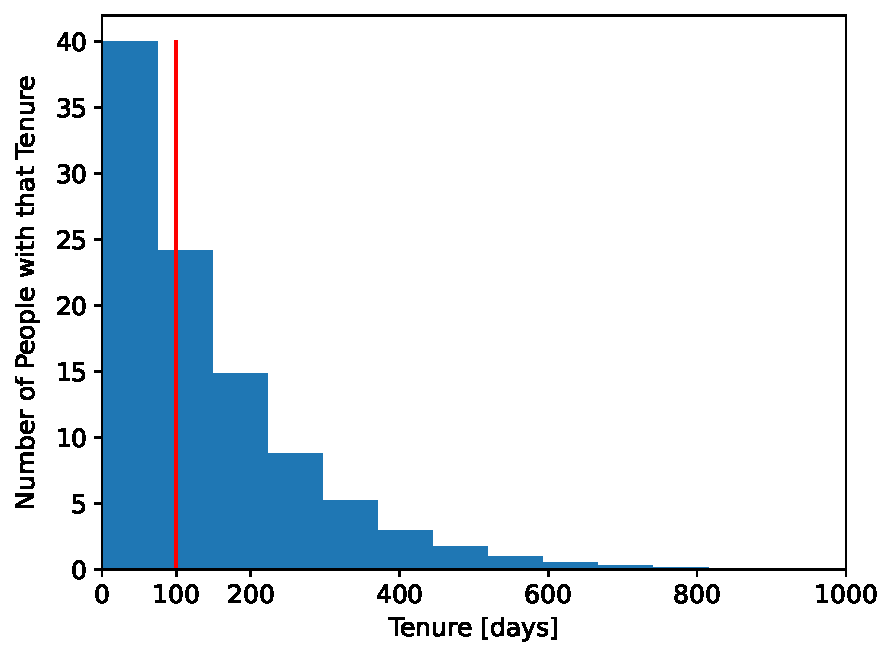
\includegraphics[width=0.8\textwidth]{images/tenure_power_distribution_a5_with_max_tenure10_and_5_participants.pdf}
    \caption{With power law distribution of tenure, a=5,
the median tenure of the youngest participant
 in a process with 5 people is 98 days.}
    \label{fig:tenure-powerlaw-5-participants-tenure10}
\end{figure}


Three calendar months (or 70 business days) may be inadequate for complex processes or processes that are infrequent (quarterly or annual), especially if there was no training. When the number of participants is 10 people, then the median tenure of the youngest participant is 51 calendar days (37 business days).


To recap, the assumption made were
\begin{itemize}
    \item Random independent sampling of organization members. 
    \item Tenure in role matters, not tenure in organization. (Excludes transfer learning among roles.)
    \item Tenure in role fits power law distribution.
    \item The power law distribution is characterized by (a=5, max tenure=10 years). 
    \item There are 5 people involved in the process.
\end{itemize}
If that last parameter is varied, the 3 month estimate is reasonable for processes with 5 or more participants.

\begin{figure}[H]
    \centering
    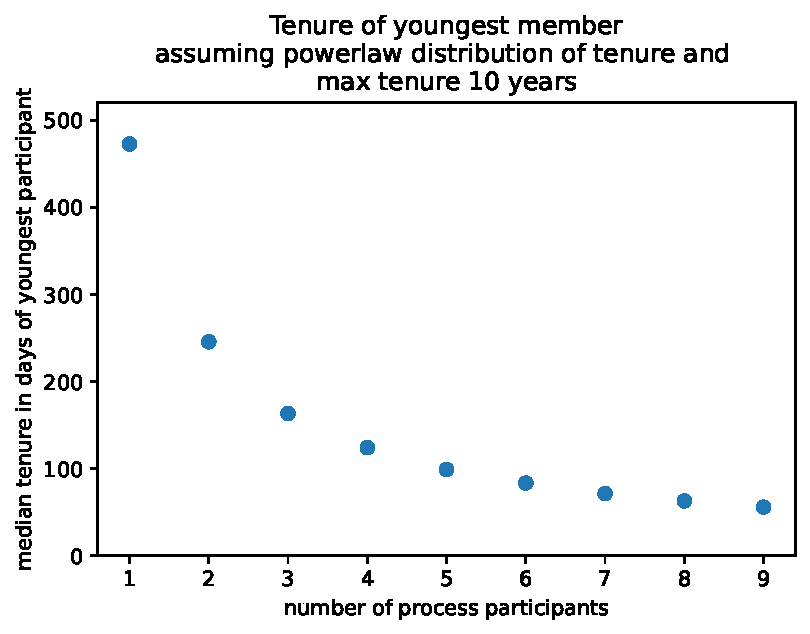
\includegraphics[width=0.8\textwidth]{images/tenure_power_distribution_a5_with_max_tenure10.pdf}
    \caption{Median tenure of the youngest participant (in calendar days) as a function of the number of process participants with tenure following a power law distribution, a=5, and max tenure = 10 years.}
    \label{fig:tenure-powerlaw-5-participants}
\end{figure}


Even when there's a single participant, the median tenure is less than 2 years because of the power law distribution of tenure.

% Uniform Distribution of Tenure instead of a Power Law Distribution
What if the power law distribution of tenure were replaced with a uniform distribution?
Surprisingly the shape of the distribution of youngest participant's tenure is not uniform, see Figure~\ref{fig:tenure-uniform-5-participants}

\begin{figure}[H]
    \centering
    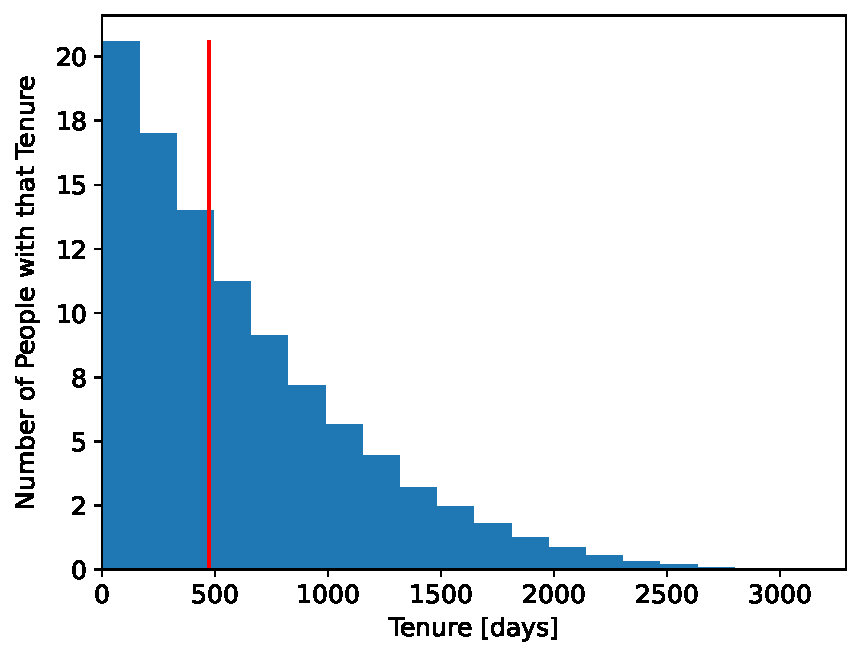
\includegraphics[width=0.8\textwidth]{images/tenure_uniform_distribution_with_max_tenure10_and_5_participants_median472.pdf}
    \caption{With uniform distribution of tenure,
the median tenure of the youngest participant
 in a process with 5 people is 472 days.}
    \label{fig:tenure-uniform-5-participants}
\end{figure}

The median tenure of the youngest member of a 5 participant is 15 months. 
